\section{Analog-to-digital Converter}

As the name implies, an \emph{analog-to-digital converter}
(ADC) converts analog sound to a digital signal, like a
microphone.
\marginnote{An analog signal is continuous time and continuous
    amplitude, while a digital signal is discrete time and discrete
    amplitude}
The \emph{resolution} $N$ of an ADC is the number of binary bits
in the ADC output.

\begin{equation}
    \text{ADC Output} = round\left( (2^N - 1)\frac{V_{\text{input}}}{V_{\text{ref}}} \right)
\end{equation}

$V_{\text{ref}}$ is the maximum input voltage that can be converted by the ADC.

The least significant bit (LSB) holds the lowest value of the encoded
analog signal.
The maximum error due to quantization is
\begin{equation}
    \pm \frac{1}{2}LSB = \pm \frac{1}{2} \frac{V_\text{ref}}{2^N-1}
\end{equation}

An ADC does not have infinitely fast conversion. The \emph{sampling rate}
is the number of output samples available per unit time.

The sampling frequency needed to prevent aliasing, which causes distortion,
is given by the Nyquist-Shannon Sampling Theorem,
\begin{equation}
    f_{\text{sampling}} \geq 2f_{\text{signal}}
\end{equation}

This class focuses on \emph{successive-approximation} (SAR) ADCs,
as in Figure \ref{fig:saradc}.

\begin{figure}
    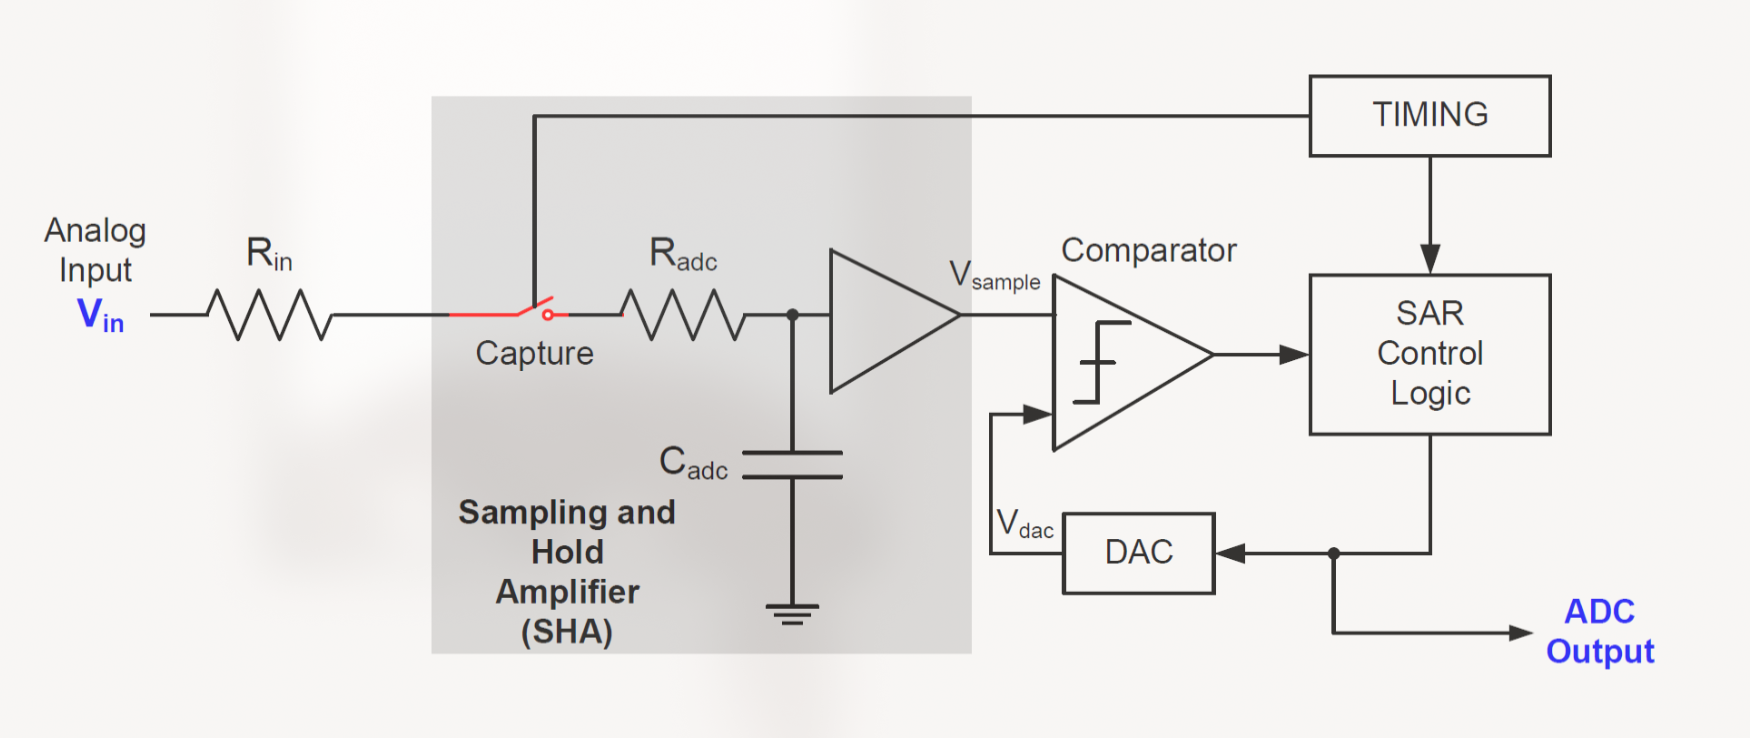
\includegraphics{images/saradc.png}
    \caption{SAR ADC}
    \label{fig:saradc}
\end{figure}

\emph{Jitter} is small rapid variations in a waveform resulting from
fluctuations in the voltage supply or mechanical vibrations or other
sources. Jitter is noise from the surroundings, from the microcontroller,
and from the ADC itself. One of the most reliable ways of defeating noise
is taking more samples than needed and averaging them out.

One type of this averaging out is called "moving window" sampling, so named
because one averages $N$ samples in a small section (window) of a signal,
then moves the window by one and repeats the process.

\begin{lstlisting}
    #define HISTSIZE 128

    int his1[HISTSIZE] = { 0 };
    int sum1 = 0;
    int pos1 = 0;
    
    int his2[HISTSIZE] = { 0 };
    int sum2 = 0;
    int pos2 = 0;

    ... 

    reading = ADC1->DR;
    sum1 -= hist1[pos1];
    sum1 += hist1[pos1] = reading;
    pos1 = (pos1 + 1) % HISTSIZE;
    val = sum1/HISTSIZE;
    sprintf(line, "%2.3f", val * 3 / 4095.0);
    display1(line);

    ADC1->CHSELR = 0;
    ADC1->CHSELR |= 1 << 5;
    while(!(ADC1->ISR & ADC_ISR_ADRDY));
    ADC1->CR |= ADC_CR_ADSTART;
    while(!(ADC1->ISR & ADC_ISR_EOC));

    reading = ADC1->DR;
    sum2 -= hist2[pos2];
    sum2 += hist2[pos2] = reading;
    pos2 = (pos2 + 1) & (HISTSIZE - 1);
    val = sum2 >> 7;
    // division is painfully slow
    // if HISTSIZE is a power of 2
    // replace divisions with a 
    // bitwise AND operation and 
    // right shift
    sprintf(line, "%2.3f", val * 3 / 4095.0);
    display2(line);
\end{lstlisting}